\documentclass[a4paper,titlepage]{article}

\usepackage{fullpage}

\usepackage[T1]{fontenc}
\usepackage[utf8]{inputenc}
\usepackage[spanish]{babel}
\usepackage{pdfpages}

\begin{document}

\title{Algorítmos y Estructuras de Datos II\\
Trabajo Práctico 1 (Especificación)\\
Grupo 6}

\author{
	Bayardo, Julián\\
	julian@bayardo.com.ar\\
	\texttt{850/13}
	\and
	Cuneo, Christian\\
	chriscuneo93@gmail.com\\
	\texttt{755/13}
	\and
	Gambaccini, Ezequiel\\
	ezequiel.gambaccini@gmail.com\\
	\texttt{715/13}
	\and
	Lebrero Rial, Ignacio Manuel\\
	ignaciolebrero@gmail.com\\
	\texttt{751/13}
}

\date{9 de Septiembre del 2014}

\maketitle

\section{Aclaraciones}

Asumimos que las estaciones, junto con las sendas y las restricciones entre ellas no son mutables: una instancia del TAD Ciudad comienza con un mapa definido y no puede ser cambiado. Suponemos también que las estaciones pueden tener sendas que las conecten a sí mismas, así como una cantidad contable de sendas que la conecten a otra estación definida, siempre y cuando sean consideradas distintas. Aparte, los robots pueden tomar cualquier senda que los una con otra estación, incluso si esa senda le agrega una infracción, y sin importar que haya otras sendas que lo unan directamente y no le agreguen infracciones (es decir, nunca se asume que el robot vaya a tomar un camino que minimice las multas). Aparte, consideramos que pueden haber estaciones no conexas, y en cuyo caso no son consideradas bloqueantes (aunque los robots en ellas no podrían moverse hacia ningún lado).

Consideramos que dos robots son equivalentes cuando su RUR (que es asignado automáticamente por el modelo) lo es. Los RUR se asignan desde el 1 de forma incremental, y nunca se repiten: si un robot es borrado por medio de una inspección, ningún otro robot va a tener el mismo RUR asignado. No puede existir un robot que no tenga ninguna característica.

Aparte, consideramos que dos sendas entre dos estaciones iguales son equivalentes cuando las restricciones impuestas sobre ellas lo son. Dos restricciones son equivalentes cuando su tabla de verdad es la misma para todo posible conjunto de características. Cabe destacar que consideramos que dos ciudades son equivalentes cuando las estaciones, sus conexiones, y el conjunto de robots en circulación, junto con su pasado, son equivalentes observacionalmente.

Cabe destacar que no modelamos el paso del tiempo, por lo que las inspecciones no son automáticas, sino que deben ser causadas deliberadamente por quien maneje el sistema.

\section{Sobre el formato}

Inicialmente escribimos la especificación utilizando UTF-8 en lugar de LaTeX, pensando que podríamos fácilmente incluir el archivo en nuestro informe, mas esto resultó ser problemático por varias cuestiones. Finalmente, optamos por incluirlo por separado como un archivo en otro pdf. Debido a problemas con esta solución, tuvimos que ajustar el texto para que no pase de 90 columnas; adoptamos una convención que es que si las precondiciones de una función superan tal tamaño, la guarda se pasa a otra linea y se indenta al mismo nivel que el tipo de la función.

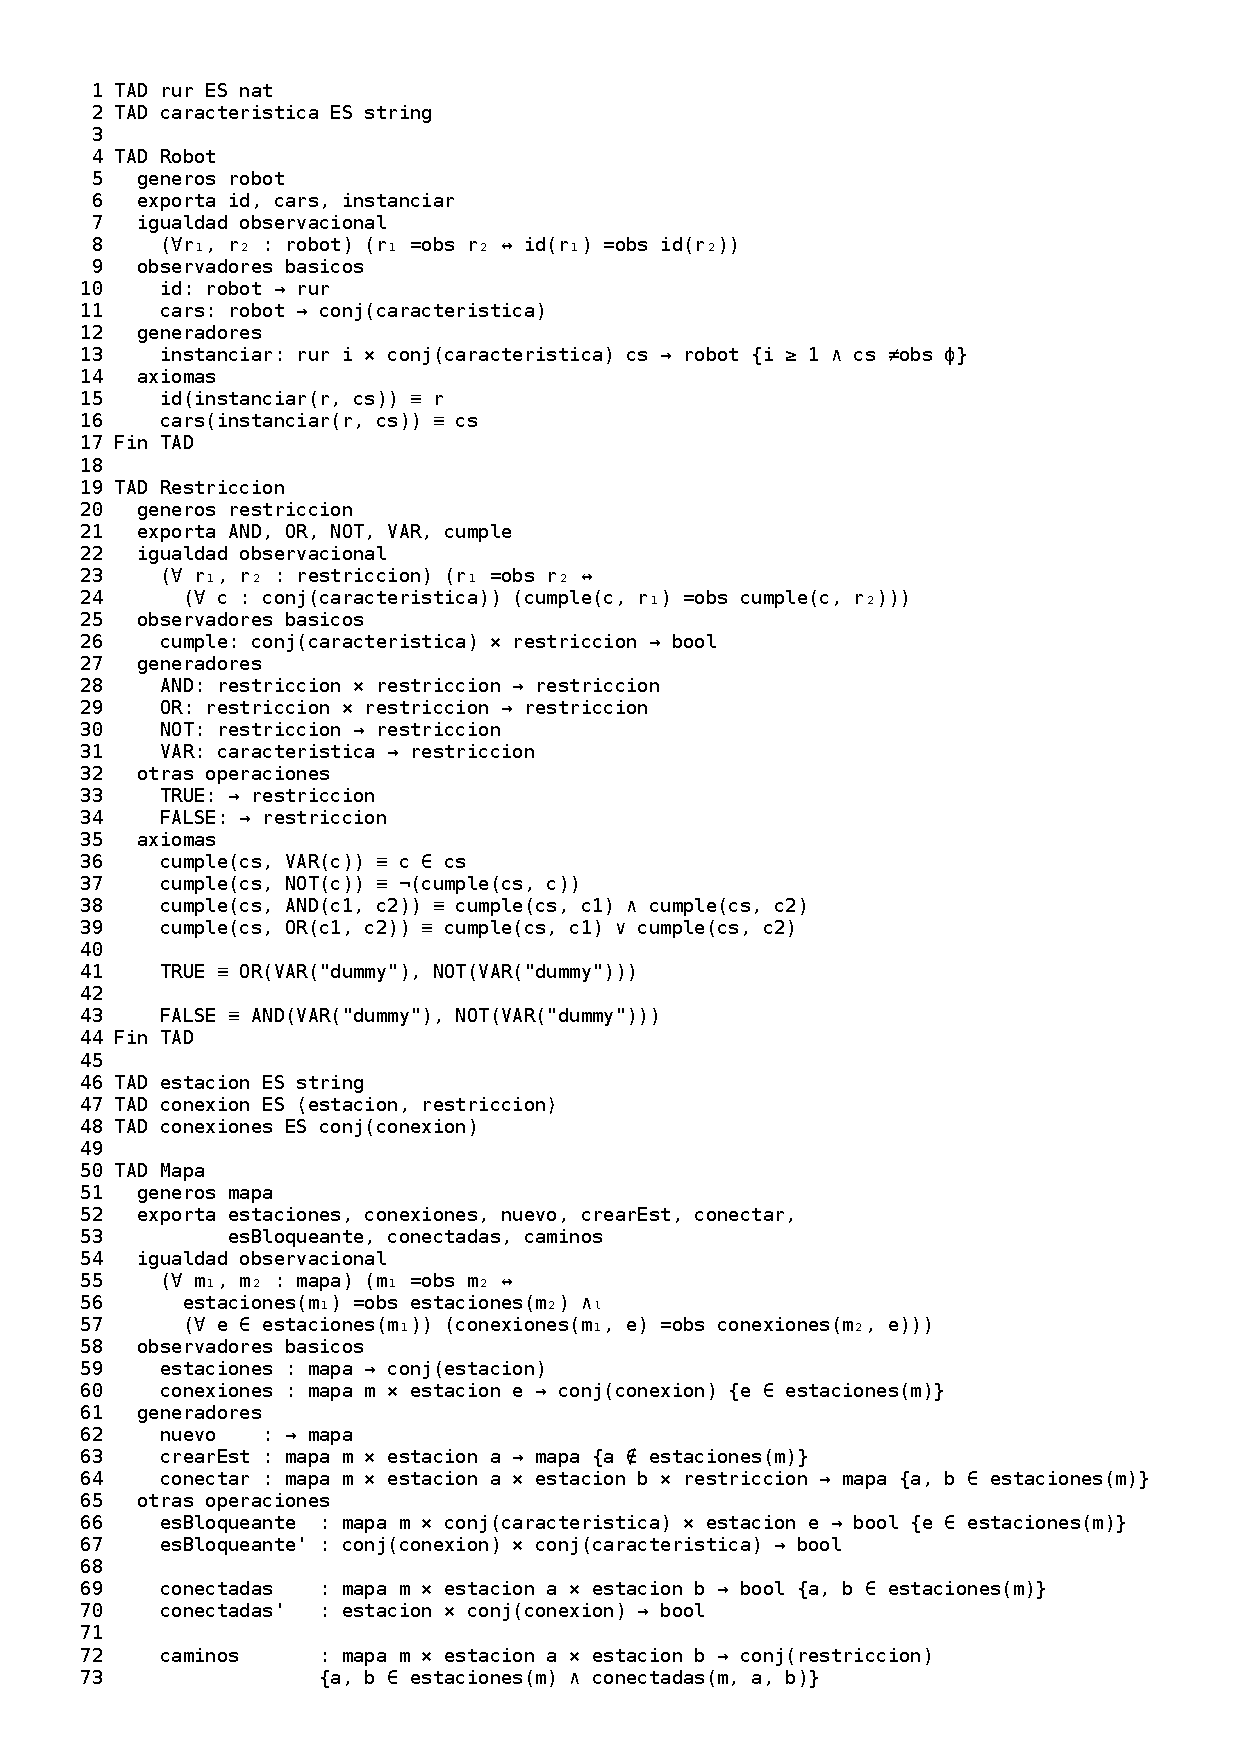
\includepdf[pages={1, 2, 3, 4}]{Especificacion.pdf}

\end{document}
